\RussianSourceFrame{GELFAND-P001425}{1}
\underline{8/II--88 г.} \underline{Сем. Гельфанда.}

И.М.Г. \underline{Задачи.} 1. Вычислить
\begin{equation*}
(1)\qquad \det\left\Vert\frac{1}{x_i-y_k}\right\Vert_{i,k=1}^{n}.
\end{equation*}
2. Док., что полином Лежандра
\begin{equation*}
\bigl((x^2-1)^n\bigr)^{(n)}
\end{equation*}
имеет только вещественные нули.

3. Может ли ф-я, являющаяся пределом непрерывных функций всюду на отрезке

а) иметь разрывы?

б) иметь всюду плотное м-во точек разрыва?

в) быть всюду разрывной (т.е. в каждой точке)?

4. \textbf{Конформно отобразить на круг}

а)\quad
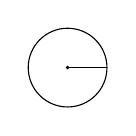
\begin{tikzpicture}[baseline=0cm]
\draw (0,0) circle (0.5);
\fill (0,0) circle (0.025);
\draw (0,0)--(0.5,0);
\end{tikzpicture}
\quad (круг без радиуса!)

б)
\begin{center}
\begin{tikzpicture}[scale=0.95]
\draw (0.645,0.08) arc (7.07:352.93:0.65)
 -- (3.355,-0.08) arc (187.07:532.93:0.65) -- cycle;
\draw[->] (0,0)--(0.23,0.60);
\node at (-0.10,0.33) {$1$};
\draw[->] (4,0)--(4.58,0.28);
\node at (4.18,0.38) {$1$};
\draw[->] (1.5,0.58)--(1.5,0.08);
\draw[->] (1.5,-0.65)--(1.5,-0.08);
\node at (1.95,0.58) {$10^{-6}$};
\fill (2.25,0) circle (0.025);
\node at (2.52,-0.24) {$A$};
\draw[->] (2.25,-0.18)--(2.25,-1.28);
\draw (2.25,-2.05) circle (0.62);
\draw[->] (2.25,-2.05)--(2.25,-1.43);
\node at (2.07,-1.72) {$1$};
\node at (2.40,-2.08) {$0$};
\node at (4.95,-1.20) {$A\mapsto\text{центр круга}$};
\end{tikzpicture}
\end{center}

\underline{\textbf{А. Бейлинсон.}} \qquad
\underline{Что нужно знать о теории струн?}

\underline{Конформная теория поля.} \qquad (2-мерная)

Операторное разложение.

Связь с представлениями естественных $\infty$-мерных алгебр Ли.

$W$-алгебры, парафермионы.

[Зачёркнуто: \RussianUnclear{GELFAND-P001425}{vertex-cancellation}{Ве\ldots{} / Вер\ldots{}}]
Алгебра \underline{Вершинных} операторов.
[Начало слова «Вершинных» переписано поверх первоначальных штрихов.]

Различные редукции предст. $\widehat{SL}_2$ к алгебре Вирасоро.

Связь с пространствами модулей алгебро-геометр. структур.

Явные формулы для стат. сумм и
[зачёркнуто: корреляционных функций; над строкой вставлено: корреляторов].

Свойство ветвления характеров.


\RussianSourceFrame{GELFAND-P001426}{unlabelled}
\underline{Д. Алексеевский.} \qquad \underline{$G$-структуры}

\underline{Скалярная полевая величина.}

[Зачёркнуто: Поле] — функция от точки $x\in\mathbb{R}^3$ с векторными значениями

(напр. со знач. в $\mathbb{R}$)

\underline{Полевая величина:} зависит от сист. координат

\underline{$G$-структура.}

\underline{Опр. 1}\quad $G\subset GL(V)$, $V=\mathbb{R}^n$.

[Под $G$:] лин. группа.

$G$-структура [вставлено над строкой: на $M^n$] — главное подрасслоение многообразия всех
[зачёркнуто: \RussianUnclear{GELFAND-P001426}{frame-prefix}{ко?}]реперов.

[Справа под «реперов»:] (кореперов) — лучше говорить.

\begin{equation*}
\begin{tikzcd}
M^{(1)} \arrow[r,"GL(V)"] & M
\end{tikzcd}
\end{equation*}
[Под $M^{(1)}$:] рассл. реперов (главное расслоение)

\begin{equation*}
\begin{tikzcd}
M^{(1)} \arrow[r,"GL(V)"] & M \\
P \arrow[u,phantom,"\cup" description] \arrow[ur,"G"'] &
\end{tikzcd}
\end{equation*}
$G$ должно действ. на $P$ транзитивно.
\RussianUnclear{GELFAND-P001426}{transitivity}{на $P$ транзитивно}

Тогда это и есть $G$-структура.

\underline{Примеры:} 1) рим. метрика — это $O(V)$-структура

2) Пусть $S$ — тенз. поле, когда оно задаёт $G$-структуру?

Если они все одного кан. вида

(в $\forall$ точке $\exists$ корепер
[зачёркнуто: \RussianUnclear{GELFAND-P001426}{tensor-cancellation}{$\theta$ / $\varphi$?}], прив. $S$ к фикс. виду)

Тогда если $G$ — гр. автоморфизмов кан. вида, то $S$ зад. $G$-структуру.

3) Аффинор зад. $G$-стр., если в $\forall$ точке одинак. жорд. форма

4) Почти компл. структура $J$: $G=GL\left(\frac{n}{2},\mathbb{C}\right)$

5) Почти симпл. структ.: 2-форма $\sigma$ макс. ранга

(симпл. стр.: $d\sigma=0$)

\underline{Опр. 2}\quad $G$-структура — главное $G$-расслоение
$\pi\colon P\overset{G}{\longrightarrow}M$

$G\subset GL(V)$

снабж. векторнозначной 1-формой $\theta\colon TP\to V$,

облад. след. условиями:


\RussianSourceFrame{GELFAND-P001427}{2}
а) $G$-эквивариантность

б) $\operatorname{Ker}\theta=T^vP$ (вертик. пр-во), т.е. $\theta$ строго горизонтальна.

\underline{Эквивалентность определений 1 и 2.}

$p\in P$, $x=\pi p$;
\begin{equation*}
\theta_p\colon T_xM\overset{\simeq}{\longrightarrow}V.
\end{equation*}
[Под $T_xM$, со скобкой и стрелкой вниз:]
\RussianUnclear{GELFAND-P001427}{quotient-notation}{$(T_pM/T_p^vM)$}.

[Справа:] это и есть корепер, с к-рым отождествляется точка $p$.

[Зачёркнуто: $\theta_p$ на \RussianUnclear{GELFAND-P001427}{zero-cancellation}{слое?} $0$.]

Корепер $\simeq$ изоморфизм $\theta_p\colon T_xM\overset{\simeq}{\longrightarrow}V$.

$\theta$ наз. \underline{формой смещения}.

Пусть есть $G$-структура
\begin{equation*}
(\pi\colon P\overset{G}{\longrightarrow}M;\theta)
\end{equation*}
Рассм. расслоение 1-струй расслоения $\pi$
\begin{equation*}
\pi'\colon P'\to P
\end{equation*}
$x\to p_x$ — сечение
\begin{equation*}
p'\colon T_xM\to T_{p_x}P
\end{equation*}
\underline{Опр.} 1-струя — отобр. $p'$ — обр. к проекции, $p'=j_x^1(p)$
\begin{equation*}
p'=j_x^1(p)\colon
\begin{tikzcd}
T_xM \arrow[r] & T_{p_x}P \arrow[l,bend left=40]
\end{tikzcd}
\end{equation*}
т.е. $\pi_*\circ p'=\mathrm{id}$

\underline{Опр.} Горизонтальное подпр-во $H\subset T_pP$
[зачёркнуто: \RussianUnclear{GELFAND-P001427}{horizontal-cancellation}{неразборчиво}]
— такое подпр-во
\begin{equation*}
T_pP=T_p^v\oplus H
\end{equation*}
\underline{Второе опр. 1-струи}

\underline{Элементы $P'$} $=$ \underline{горизонт. подпр-ва}

[Под «Элементы $P'$»:] ($=$ 1-струи)
\begin{equation*}
p'\in P'\quad\Longleftrightarrow\quad H(p')\text{ — горизонт. подпр-во}
\end{equation*}
\underline{Связь:}
\begin{equation*}
p'\colon T_xM\to H(p')\subset T_pP
\end{equation*}
\underline{Опр.} [Зачёркнуто: \RussianUnclear{GELFAND-P001427}{connection-cancellation}{$P'$?}]
$\pi'$ наз. \underline{расслоением связностей};


\RussianSourceFrame{GELFAND-P001428}{unlabelled}
\underline{Пр-во связностей:}\quad $\Gamma(\pi')^G$

(т.е. связность — это $G$-эквивар. сечение расслоения $\pi'\colon P'\to P$)

\underline{Связность:}
\begin{equation*}
\begin{aligned}
h\colon P&\to P'\\
p&\mapsto H(p)
\end{aligned}
\end{equation*}
($G$-инв. поле горизонт. подпространств)

Отсюда паралл. перенос (огранич. на кривую)

\underline{Функция кручения}\qquad (аналог структ. констант группы Ли)

Есть вертик. параллелизм:
\begin{equation*}
\begin{aligned}
i_p\colon\mathfrak g&\overset{\simeq}{\longrightarrow}T_p^vP\\
X&\mapsto X_p:=\left.\frac{d}{dt}(\exp tX)p\right|_{t=0}
\end{aligned}
\end{equation*}
\begin{equation*}
\begin{tikzcd}[column sep=small]
p'\in P'\ \Rightarrow\ T_pP={} & T_p^v \arrow[d,"i_p^{-1}"] & {}\oplus H(p') \\
\pi'(p')=p & \mathfrak g &
\end{tikzcd}
\end{equation*}
[Непосредственно после знака равенства в разложении $T_pP$ зачёркнуто:
\RussianUnclear{GELFAND-P001428}{decomposition-cancellation}{неразборчиво}.]

Возьмём форму $\theta_p\colon T_pP\to V$

и положим
\begin{equation*}
\theta_{H(p')}=\theta|_{H(p')}\colon H(p')\overset{\simeq}{\longrightarrow}V
\end{equation*}
\underline{Опр.}\quad \underline{ф-я кручения} — это отображение
\begin{equation*}
t\colon P'\longrightarrow\operatorname{Hom}(V\wedge V,V)
\end{equation*}
(тензоры типа 1,2)
\begin{equation*}
p'\mapsto t_{p'},\qquad
 t_{p'}(\xi,\eta)=d\theta\bigl(\theta_{H(p')}^{-1}\xi,\theta_{H(p')}^{-1}\eta\bigr)
\end{equation*}
\underline{Свойства ф-и кручения.}

1) $G$-эквивариантность и $G'=\operatorname{Hom}(V,\mathfrak g)$-эквивариантность


\RussianSourceFrame{GELFAND-P001429}{3}
\underline{15/II--88 г.}\qquad \underline{Сем. Гельфанда}
(по записям А.К. Звонкина)

В лекциях И.М.Г. о квазилинейных уравнениях (УМН--59, т.14, № 2)
на трёх страницах изложена \underline{вся термодинамика}.

\underline{Конкр. зад. по геометрии:} что такое угол между двумя 2-мерными подпр-вами
в 4-мерном пр-ве?

Угол — инвариант относит. дв-ния (для прямых).

Есть 2 варианта: для ориентир. прямых и для неориентированных.

Для плоскостей: сколько этих инвариантов и каковы они?

\underline{Вопрос:} найти все инварианты двух подпространств гильбертова пространства.

[Зачёркнуто: \RussianUnclear{GELFAND-P001429}{speaker-cancellation}{Зам\ldots{}?}]

\underline{Замолодчиков Саша.}\qquad
\underline{Конформная (2-мерная) теория поля.}

\begin{equation*}
\langle A_1(x_1)A_2(x_2)\ldots A_N(x_N)\rangle,\quad x_i\in\mathbb{R}^2;
\tag{1}
\end{equation*}
— «корреляционные функции»

$\mathcal A\ni A$ — поля (вообще говоря, $\infty$-мерное)

(1) — $N$-линейная ф-я на пр-ве полей $\mathcal A$
(к тому же ф-я от $(x_1,\ldots,x_N)$)

Уточним понятие среднего в (1):
\begin{equation*}
(1)=Z^{-1}\int\mathcal D\varphi\,e^{-S[\varphi]}A_1(x_1)\ldots A_N(x_N),
\tag{2}
\end{equation*}
где $\varphi=\varphi(x)$,
\begin{equation*}
S=\int\sigma\bigl(\varphi(x),\partial\varphi(x)\bigr)\,dx,
\tag{3}
\end{equation*}
\begin{equation*}
Z=\int\mathcal D\varphi\,e^{-S[\varphi]}
\tag{4}
\end{equation*}
[Номер (4) переписан поверх \RussianUnclear{GELFAND-P001429}{equation-number}{3?}.]

\underline{Свойства корреляционных функций.}

1) «Алгебра полей»

Пусть поля образуют ассоц. алгебру;
[зачёркнуто: \RussianUnclear{GELFAND-P001429}{algebra-cancellation}{неразборчиво}]
с \RussianUnclear{GELFAND-P001429}{algebra-ending}{образующими / образующих} $A_i(x)$.
[Над строкой вставлено: (с континуумом); окончание слова «образующими» исправлено.]

Пусть $\{A_i\}$ — базис в $\mathcal A$. Тогда
\begin{equation*}
A_i(x)A_j(y)=\sum_k c_{ij}^k(x,y)A_k(y)
\end{equation*}
[К $c_{ij}^k(x,y)$ проведена стрелка от подписи:] числовые ф-и от $x,y$

Положим
\begin{equation*}
\langle A_k(x)\rangle=a_k(x)
\end{equation*}


\RussianSourceFrame{GELFAND-P001430}{unlabelled}
(Знания функций $c_{ij}^k$ и $a_k$ достаточно для вычисления корреляц.
функций: заменяем пару $A_1A_2$ на $\sum c^kA_k$ и т.д.)

2) \underline{«Инвариантность»}

Рассм. поле $T$ вида
\begin{equation*}
T^{\mu\nu},\quad\mu,\nu=1,2;\quad T^{\mu\nu}\in\mathcal A.
\end{equation*}
Кстати
\begin{equation*}
\frac{\partial}{\partial x^\mu}A_i(x)A_j(y)
=\sum\frac{\partial}{\partial x^\mu}c_{ij}^k(x,y)A_k
\tag{5}
\end{equation*}
\begin{equation*}
\frac{\partial T^{\mu\nu}}{\partial x^\mu}=0
\tag{6}
\end{equation*}
Рассм. [зачёркнуто: \RussianUnclear{GELFAND-P001430}{integral-cancellation}{оператор?}] интеграл
\begin{equation*}
\oint T^{\mu\nu}(x)A(y)\,\varepsilon_{\mu\lambda}\,dx^\lambda
\tag{7}
\end{equation*}
[Индекс $\lambda$ у $\varepsilon$ переписан поверх
\RussianUnclear{GELFAND-P001430}{epsilon-first-index}{$\nu$?}.]

[Справа от интеграла:]
\begin{center}
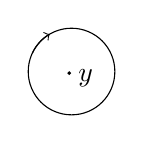
\begin{tikzpicture}
\draw (0,0) circle (0.55);
\draw[->] (155:0.55) arc (155:120:0.55);
\fill (-0.03,-0.02) circle (0.025);
\node at (0.18,-0.08) {$y$};
\end{tikzpicture}
\end{center}
[Выносная подпись к $\varepsilon$ в (7):]
\begin{equation*}
\varepsilon_{\mu\lambda}=-\varepsilon_{\lambda\mu},\qquad\varepsilon_{12}=1
\end{equation*}
Он определяет линейный оператор в $\mathcal A$.

\underline{Требуется:} $\exists$ поле $T$ такое, что этот оператор равен $\dfrac{\partial}{\partial y}$.

$T^{\mu\nu}:=$ «тензор энергии-импульса»
\begin{equation*}
\oint T^{\mu\nu}(x)A_i(y)\,
\varepsilon_{\mu\nu}
\,dx^\lambda
=\frac{\partial}{\partial y^\nu}A_i(y)
\end{equation*}
\RussianUnclear{GELFAND-P001430}{epsilon-repeat}{$\varepsilon_{\mu\nu}$}
$1')$\quad $c_{ij}^k(x,y)=c_{ij}^k(x-y)$ — функции одной переменной в $\mathbb R^2$.

3) \underline{«Условие положительности»}

$A\mapsto A^+\in\mathcal A$ — инволюция.
\begin{equation*}
A_i^+(x)A_j^+(y)=\sum\overline{c}_{ij}^k(\widetilde x-\widetilde y)A_k^+(y)
\tag{8}
\end{equation*}
\begin{equation*}
x=(x^1,x^2)\quad\Rightarrow\quad\widetilde x=(-x^1,x^2)
\end{equation*}
\underline{Требование:} матрица $\langle A_i^+(\widetilde x)A_j(x)\rangle$
положительно определена для всех $x$.

\underline{Задача} состоит в том, чтобы строить содержательные примеры всего этого.


\RussianSourceFrame{GELFAND-P001431}{4}
Введём в $\mathbb R^2$ комплексные координаты
\begin{equation*}
z=x^1+ix^2\qquad ds^2=dz\,d\bar z
\end{equation*}
\begin{equation*}
T^{\nu\mu}=T^{\mu\nu}
\tag{9}
\end{equation*}
\begin{equation*}
\left.\begin{aligned}
T&=T^{zz},\quad\bar T=T^{\bar z\bar z}\\
\Theta&=T^{z\bar z}=0
\end{aligned}\right\}
\quad\begin{gathered}
\text{при этих дополнительных условиях}\\
\text{теория наз. «конформной теорией поля»}
\end{gathered}
\tag{10}
\end{equation*}
\RussianUnclear{GELFAND-P001431}{tensor-components}{$T=T^{zz},\ \bar T=T^{\bar z\bar z}$}

[Стрелка снизу к $\Theta=0$:] Важн. частный случай: безмассовая теория

\underline{Контр. вопрос:} записать $T^{zz}$, $T^{z\bar z}$, $T^{\bar z\bar z}$ через $T^{\mu\nu}$

(это задача линейной алгебры)
\begin{equation*}
\frac{\partial T}{\partial\bar z}=0,\quad
\frac{\partial\bar T}{\partial z}=0
\qquad\text{— уравнения Коши--Римана}
\tag{11}
\end{equation*}
\begin{equation*}
\Updownarrow
\end{equation*}
$T$ — аналитическая функция $z$, $T=T(z)$, $\bar T=\bar T(\bar z)$.
\begin{equation*}
T(z)A_i(z_1,\bar z_1)=\sum f_{ij}(z-z_1)A_j(z_1,\bar z_1)
\tag{12}
\end{equation*}
\underline{В электродинамике:}

$\psi$ — электрон

$A$ — фотон
\begin{equation*}
\{A_i\}=\{\psi,\psi^2,\psi\partial\psi,\ldots,A,A^2,A\psi,\ldots\}
\end{equation*}
$\psi^4$ ещё есть, но $\psi^5=\psi^6=0$ (т.к. всего у спинора 4 компоненты)

у $A$ есть все степени

Но, вообще говоря, $A^2$ не существует.

Не надо брать поля в одной точке, надо в разных.
\begin{equation*}
\oint\frac{dz}{2\pi i}\,z^{n+1}T(z)A_i(z_1,\bar z_1)
=L_nA_i(z_1,\bar z_1)
\tag{13}
\end{equation*}
[Справа от (13):]
\begin{center}
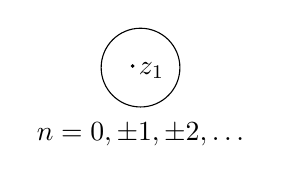
\begin{tikzpicture}
\draw (0,0) circle (0.5);
\fill (-0.10,0.02) circle (0.025);
\node at (0.14,-0.04) {$z_1$};
\node at (0,-0.85) {$n=0,\pm1,\pm2,\ldots$};
\end{tikzpicture}
\end{center}
\begin{equation*}
L_{-1}=\frac{\partial}{\partial z_1}
\end{equation*}
\begin{equation*}
\bar T(\bar z)\to\bar L_n;\quad
\bar L_{-1}=\frac{\partial}{\partial\bar z_1}
\tag{14}
\end{equation*}
$T(z_1)T(z_2)$ — ф-я от $z_1$, аналитическая везде, кроме точки $z_2$;
разложим её в ряд Лорана.


\RussianSourceFrame{GELFAND-P001432}{unlabelled}
\begin{equation*}
T(z_1)T(z_2)=\sum_{m=-\infty}^{\infty}(z_1-z_2)^m T_m(z_2),\quad T_m\in\mathcal A
\tag{15}
\end{equation*}
Сделаем предположение:
\begin{equation*}
(15)=(z_1-z_2)^{-4}T_{-4}+(z-z_2)^{-3}T_{-3}+\ldots
\tag{16}
\end{equation*}
\RussianUnclear{GELFAND-P001432}{laurent-factor}{$(z-z_2)^{-3}$}

(т.е. ряд обрывается внизу на члене $-4$)
\begin{equation*}
T_{-1}=\frac{dT}{dz_2}(z_2)
\tag{17}
\end{equation*}
\begin{equation*}
T_{-2}=2T(z_2)\quad\leftarrow\quad
\text{выводится из того, что $T$ — тензор 2-го ранга}
\tag{18}
\end{equation*}
Важнее всего определить самые сингулярные слагаемые: $T_{-3}$ и $T_{-4}$.

Из условия положительности следует, что
\begin{equation*}
T_{-4}\sim\text{единичн. оператор:}\quad T_{-4}=\frac c2,\quad T_{-3}=0
\tag{19}
\end{equation*}
\begin{equation*}
T(z)T(z')=\frac{c}{2(z-z')^4}+\frac{2T(z')}{(z-z')^2}
+\frac{1}{z-z'}T'(z')+\ldots
\tag{20}
\end{equation*}
[Стрелка к многоточию в (20):] дальнейшие члены не интересны

Из этого разложения получаем
\begin{equation*}
\fbox{$[L_n,L_m]=(n-m)L_{n+m}+\frac{c}{12}(n^3-n)\delta_{n+m,0}$}
\tag{21}
\end{equation*}
Это соотн. \underline{алгебры Вирасоро} (центр. расширение алгебры векторных полей на окружности)

(В обычной квантовой механике — алгебра Ли группы параллельных переносов на прямой: $\frac{d}{dx}$ — малый перенос — импульс)

Вообще тензор энергии-импульса получается из преобразований координат

В этом смысле квантовую механику придумал Софус Ли: он первый заменил преобразования координат на беск. малые преобразования.

(Для алгебры Вирасоро группой служит группа диффеоморфизмов окружности.)

Длины меньше $10^{-31}$ см не имеют смысла — это утверждение уже не зависит
[зачёркнуто: \RussianUnclear{GELFAND-P001432}{lower-cancellation}{от / не}]
ни от какой теории — из соотношений между универсальными константами.


\RussianSourceFrame{GELFAND-P001433}{5}
$p$-адическая теория имеет вычислительные преимущества: некоторые детерминанты лучше всего считать адельным способом

Но есть и ещё одно: физика ничего не может сказать не только о далёких точках, но и о близких.

[Следующий абзац выделен двумя вертикальными чертами слева:]
О двумерных многообразиях всё известно, но о трёхмерных и четырехмерных известно столь же мало, как и 2000 лет назад

Это новая комбинаторика.

Как придумать, что такое пространство, если есть запрет на малые расстояния? Не хватает воображения. (Толщина; дискретность; искривления;\ldots)

[Короткая горизонтальная черта.]

Конформная инвариантность: теория не меняется при замене
\begin{equation*}
\begin{cases}
z\mapsto z+\varepsilon(z)\\
\bar z\mapsto\bar z+\bar\varepsilon(\bar z)
\end{cases}
\tag{22}
\end{equation*}
Взяв $\varepsilon(z)\sim z^{n+1}$, получим алгебру Вирасоро

Выясним, как меняется среднее
\begin{equation*}
\langle A_1(x_1)\ldots A_N(x_N)\rangle
=Z^{-1}\int A_1(x_1)\ldots A_N(x_N)e^{-S[\varphi]}\mathcal D\varphi
\tag{23}
\end{equation*}
при заменах
\begin{equation*}
x^\mu\to x^\mu+\varepsilon^\mu(x)
\tag{24}
\end{equation*}
Вариация
\begin{equation*}
\begin{aligned}
\delta\langle A_1(x_1)\ldots A_N(x_N)\rangle
&=\sum_{k=1}^{N}\langle A_1\ldots\delta_\varepsilon A_k\ldots A_N\rangle\\
&\quad+\int\partial_\mu\varepsilon_\nu
\langle T^{\mu\nu}(x)A_1\ldots A_N\rangle\,d^2x=0
\end{aligned}
\tag{25}
\end{equation*}
перебросим (по частям) $\partial_\mu$ на $T^{\mu\nu}$ и воспольз. $\partial_\mu T^{\mu\nu}=0$;

интегрир. по маленьким контурам, окруж. $x_1,\ldots,x_N$, получим
\begin{equation*}
\delta_\varepsilon A_k(y)=\oint_{c_y}\varepsilon_\nu(x)T^{\lambda\nu}(x)
\varepsilon_{\lambda\mu}\,dx^\mu A_k(y),
\end{equation*}
но
\begin{equation*}
\partial_\mu\varepsilon_\nu+\partial_\nu\varepsilon_\mu=\delta_{\mu\nu}\rho(x);
\end{equation*}
\RussianUnclear{GELFAND-P001433}{conformal-factor}{$\rho(x)$ / $g(x)$}

$T^{z\bar z}=T^\mu_\mu$ — след; $=0$.
\RussianUnclear{GELFAND-P001433}{trace-equality}{$T^{z\bar z}=T^\mu_\mu$}

[Внизу справа:]
\begin{center}
\begin{tikzpicture}
\node[align=left] at (0,0) {Что\\получилось};
\draw (1.7,0) ellipse (0.35 and 0.45);
\node at (1.7,0) {?};
\end{tikzpicture}
\end{center}


\RussianSourceFrame{GELFAND-P001434}{unlabelled}
Поля классифицируются по представлениям алгебры Вирасоро.
\begin{equation*}
\left\{\begin{aligned}
L_n\phi_\alpha&=0,\quad n>0;&\qquad\bar L_n\phi_\alpha&=0;\\
L_0\phi_\alpha&=\Delta_\alpha\phi_\alpha;&\qquad
\bar L_0\phi_\alpha&=\bar\Delta_\alpha\phi_\alpha;
\end{aligned}\right.
\tag{26}
\end{equation*}
\begin{equation*}
L_{n_N}\ldots L_{n_1}\phi_\alpha=[\phi_\alpha]
\end{equation*}
\RussianUnclear{GELFAND-P001434}{descendant-bracket}{$L_{n_N}\ldots L_{n_1}\phi_\alpha=[\phi_\alpha]$}
\begin{equation*}
n_i<0;\quad\Delta_\alpha,\bar\Delta_\alpha\text{ — два числа }\geq0
\end{equation*}
\begin{equation*}
\mathcal A=\bigoplus_\alpha[\Phi_\alpha]
\end{equation*}
\begin{equation*}
\mathrm I\in\mathcal A;\qquad\mathrm I\cdot A_i(x)=A_i(x),\quad
\text{для него }\Delta,\bar\Delta=0
\end{equation*}
\begin{equation*}
\begin{gathered}
z\to\lambda z\\
\bar z\to\bar\lambda z
\end{gathered}
\qquad\phi_\alpha\to\lambda^{\Delta_\alpha}\bar\lambda^{\bar\Delta_\alpha}\phi_\alpha,
\end{equation*}
\RussianUnclear{GELFAND-P001434}{barred-coordinate}{$\bar z\to\bar\lambda z$}
\begin{equation*}
\Delta_\alpha-\bar\Delta_\alpha=S_\alpha\text{ — спин }\phi_\alpha.
\end{equation*}

